\documentclass[12pt]{article}
\usepackage{latexsym,amssymb,amsmath} % for \Box, \mathbb, split, etc.
% \usepackage[]{showkeys} % shows label names
\usepackage{cite} % sorts citation numbers appropriately
\usepackage{path}
\usepackage{url}
\usepackage{verbatim}
\usepackage{float}
\usepackage{subfig}
\usepackage[pdftex]{graphicx}

% horizontal margins: 1.0 + 6.5 + 1.0 = 8.5
\setlength{\oddsidemargin}{0.0in}
\setlength{\textwidth}{6.5in}
% vertical margins: 1.0 + 9.0 + 1.0 = 11.0
\setlength{\topmargin}{0.0in}
\setlength{\headheight}{12pt}
\setlength{\headsep}{13pt}
\setlength{\textheight}{625pt}
\setlength{\footskip}{24pt}

\renewcommand{\textfraction}{0.10}
\renewcommand{\topfraction}{0.85}
\renewcommand{\bottomfraction}{0.85}
\renewcommand{\floatpagefraction}{0.90}

\makeatletter
\setlength{\arraycolsep}{2\p@} % make spaces around "=" in eqnarray smaller
\makeatother

% change equation, table, figure numbers to be counted inside a section:
\numberwithin{equation}{section}
\numberwithin{table}{section}
\numberwithin{figure}{section}

% begin of personal macros
\newcommand{\half}{{\textstyle \frac{1}{2}}}
\newcommand{\eps}{\varepsilon}
\newcommand{\myth}{\vartheta}
\newcommand{\myphi}{\varphi}

\newcommand{\IN}{\mathbb{N}}
\newcommand{\IZ}{\mathbb{Z}}
\newcommand{\IQ}{\mathbb{Q}}
\newcommand{\IR}{\mathbb{R}}
\newcommand{\IC}{\mathbb{C}}
\newcommand{\Real}[1]{\mathrm{Re}\left({#1}\right)}
\newcommand{\Imag}[1]{\mathrm{Im}\left({#1}\right)}

\newcommand{\norm}[2]{\|{#1}\|_{{}_{#2}}}
\newcommand{\abs}[1]{\left|{#1}\right|}
\newcommand{\ip}[2]{\left\langle {#1}, {#2} \right\rangle}
\newcommand{\der}[2]{\frac{\partial {#1}}{\partial {#2}}}
\newcommand{\dder}[2]{\frac{\partial^2 {#1}}{\partial {#2}^2}}

\newcommand{\nn}{\mathbf{n}}
\newcommand{\xx}{\mathbf{x}}
\newcommand{\uu}{\mathbf{u}}

\newcommand{\junk}[1]{{}}

% set two lengths for the includegraphics commands used to import the plots:
\newlength{\fwtwo} \setlength{\fwtwo}{0.45\textwidth}
% end of personal macros

\begin{document}
\DeclareGraphicsExtensions{.jpg}

\begin{center}
\textbf{\Large Evaluation of Machine Learning Techniques in a Crop/Weed Image Dataset\newline(Machine Learning Final Project)} \\[6pt]
%\textbf{\Large Crop rows segmentation in sugarcane fields through computer vision techniques \newline \newline  Pattern Recognition Final Project} \\[6pt]
  Fabio Andres Herrera \\[6pt]
  Escuela de Ingeniería de Sistemas y Computación\\
  Universidad del Valle, Cali - Colombia  \\[6pt]
  fabio.herrera@correounivalle.edu.co
  %, \url{www.math.umbc.edu/~gobbert}
\end{center}

\begin{abstract}
\noindent	
This paper presents a simple academic evaluation of some machine learning (supervised and unsupervised) techniques using a computer vision approach applied to a dataset of top-down looking images of row cultures (organic carrots). The dataset comprises 60 images with annotations with a ground truth vegetation segmentation mask and manual annotation of the plant type (crop vs. weed).


\end{abstract}

\subparagraph{\textit{Key words.}}\textit{Computer Vision, Machine Learning, Phenotyping, Precision Agriculture}



\section{Introduction}

Machine learning is the science of getting computers to act without being explicitly programmed\cite{5392560}. Machine learning is about learning to do better in the future based on what was experienced in the past. The emphasis of machine learning is on automatic methods. In other words, the goal is to devise learning algorithms that do the learning automatically without human intervention or assistance. The process of learning begins with observations or data, such as examples, direct experience, or instruction, in order to look for patterns in data and make better decisions in the future based on the examples that we provide. The primary aim is to allow the computers learn automatically without human intervention or assistance and adjust actions accordingly. Machine learning is a core subarea of artificial intelligence. Machine learning algorithms are often categorized as supervised or unsupervised.


\subsection{Supervised machine learning }

Supervised machine learning algorithms can apply what has been learned in the past to new data using labeled examples to predict future events. Starting from the analysis of a known training dataset, the learning algorithm produces an inferred function to make predictions about the output values. The system is able to provide targets for any new input after sufficient training. The learning algorithm can also compare its output with the correct, intended output and find errors in order to modify the model accordingly.

\subsection{Unsupervised machine learning }

In contrast, unsupervised machine learning algorithms are used when the information used to train is neither classified nor labeled. Unsupervised learning studies how systems can infer a function to describe a hidden structure from unlabeled data. The system doesn’t figure out the right output, but it explores the data and can draw inferences from datasets to describe hidden structures from unlabeled data.

\subsection{Semi-supervised machine learning }

 fall somewhere in between supervised and unsupervised learning, since they use both labeled and unlabeled data for training – typically a small amount of labeled data and a large amount of unlabeled data. The systems that use this method are able to considerably improve learning accuracy. Usually, semi-supervised learning is chosen when the acquired labeled data requires skilled and relevant resources in order to train it / learn from it. Otherwise, acquiringunlabeled data generally doesn’t require additional resources.
 
\subsection{Reinforcement machine learning }
Is a learning method that interacts with its environment by producing actions and discovers errors or rewards. Trial and error search and delayed reward are the most relevant characteristics of reinforcement learning. This method allows machines and software agents to automatically determine the ideal behavior within a specific context in order to maximize its performance. Simple reward feedback is required for the agent to learn which action is best; this is known as the reinforcement signal.


Machine learning enables analysis of massive quantities of data. While it generally delivers faster, more accurate results in order to identify profitable opportunities or dangerous risks, it may also require additional time and resources to train it properly. Combining machine learning with AI and cognitive technologies can make it even more effective in processing large volumes of information.


\subsection{Image Dataset}

The dataset comprises field images in top-down view that were acquired with the autonomous field robot Bonirob in an organic carrot farm in 2013. The images were captured while the crop was in growth stages where one
or more true leaves were present. Some hours after data acquisition the farmer applied manual weed control on this field. Here we consider organic carrots, however similar manual weed control activities are also required for chicory, onions and other cultures. All images are annotated and a ground truth vegetation segmentation mask is available together with crop /weed annotations. Section 3 provides more details about the data, metadata and acquisition conditions


\begin{figure}[H] \centering
	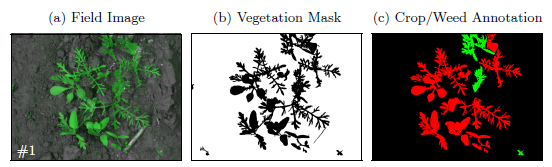
\includegraphics[width=1\textwidth]{image1.png}
	\caption{Sample images from the dataset (a) with ground truth vegetation masks
		and crop /weed annotations. The annotation images (b) and (c) are supplied for
		every image of the dataset. Best viewed in color. Modified from \cite{Haug2015}. }
	\label{figure1}
\end{figure}


\begin{figure}[H] \centering
	\caption{Description of camera system and acquisition parameters. Modified from \cite{Haug2015}. }
	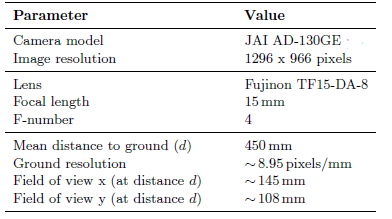
\includegraphics[width=0.6\textwidth]{image2.png}
	\label{figure2}
\end{figure}


\subsection{File metadata}




\cite{Haug2015}







\section{Bag of Words (BoW)} \label{bow}

To represent an image using the BoW model, an image can be treated as a document. Similarly, "words" in images need to be defined too. To achieve this, it usually includes following three steps: feature detection, feature description, and codebook generation. A definition of the BoW model can be the "histogram representation based on independent features".

\textbf{Feature representation}
After feature detection, each image is abstracted by several local patches. Feature representation methods deal with how to represent the patches as numerical vectors. These vectors are called feature descriptors. A good descriptor should have the ability to handle intensity, rotation, scale and affine variations to some extent. One of the most famous descriptors is Scale-invariant feature transform (SIFT). SIFT converts each patch to 128-dimensional vector. After this step, each image is a collection of vectors of the same dimension (128 for SIFT), where the order of different vectors is of no importance.

\textbf{Codebook generation}
The final step for the BoW model is to convert vector-represented patches to "codewords" (analogous to words in text documents), which also produces a "codebook" (analogy to a word dictionary). A codeword can be considered as a representative of several similar patches. One simple method is performing k-means clustering over all the vectors.Codewords are then defined as the centers of the learned clusters. The number of the clusters is the codebook size (analogous to the size of the word dictionary).

Thus, each patch in an image is mapped to a certain codeword through the clustering process and the image can be represented by the histogram of the codewords.





\subsection{Neural Networks}

%\begin{figure}[H] \centering
%	\includegraphics[width=0.9\textwidth]{image7.png}
%	\caption{Feed-forward networks (left) and Recurrent neural networks (right) .  Taken from  }
%	\label{figre7}
%\end{figure}
%image credit 	http://mesin-belajar.blogspot.com/2016/01/a-brief-history-of-neural-nets-and-deep_84.html


\subsection{Convolutional Neural Networks}


\subsection{Deep Learning}
%https://es.slideshare.net/yuhuang/deep-learning-for-image-denoising-superresolution-27435126

\subsection{Ensemble learning}
Ensemble methods use multiple learning algorithms to obtain better predictive performance than could be obtained from any of the constituent learning algorithms alone. Unlike a statistical ensemble in statistical mechanics, which is usually infinite, a machine learning ensemble consists of only a concrete finite set of alternative models, but typically allows for much more flexible structure to exist among those alternatives.

An ensemble is itself a supervised learning algorithm, because it can be trained and then used to make predictions. The trained ensemble, therefore, represents a single hypothesis. This hypothesis, however, is not necessarily contained within the hypothesis space of the models from which it is built. Thus, ensembles can be shown to have more flexibility in the functions they can represent. This flexibility can, in theory, enable them to over-fit the training data more than a single model would, but in practice, some ensemble techniques (especially bagging) tend to reduce problems related to over-fitting of the training data.

Empirically, ensembles tend to yield better results when there is a significant diversity among the models.[4][5] Many ensemble methods, therefore, seek to promote diversity among the models they combine.[6][7] Although perhaps non-intuitive, more random algorithms (like random decision trees) can be used to produce a stronger ensemble than very deliberate algorithms (like entropy-reducing decision trees).[8] Using a variety of strong learning algorithms, however, has been shown to be more effective than using techniques that attempt to dumb-down the models in order to promote diversity.[9]

\subsection{Network depth}

Network depth is of crucial importance in neural network architectures, but deeper networks are more difficult to train. The residual learning framework eases the training of these networks, and enables them to be substantially deeper — leading to improved performance in both visual and non-visual tasks. These residual networks are much deeper than their ‘plain’ counterparts, yet they require a similar number of parameters (weights).

\subsection{Residual Learning}

In general, in a deep convolutional neural network, several layers are stacked and are trained to the task at hand. The network learns several low/mid/high level features at the end of its layers. In residual learning, instead of trying to learn some features, we try to learn some residual. Residual can be simply understood as subtraction of feature learned from input of that layer. ResNet does this using shortcut connections (directly connecting input of nth layer to some $(n+x)th$ layer. It has proved that training this form of networks is easier than training simple deep convolutional neural networks and also the problem of degrading accuracy is resolved


%\subsection{Example} \label{subsecexample}
%
%We know that the error of the finite difference approximation using
%\begin{figure} \centering
%  \includegraphics[width=0.5\textwidth]{mesh_solution}
%  \caption{Solution to test problem with $h = 1 / 32$.}
%  \label{figsolplot}
%\end{figure}
%centered differences for an elliptic partial differential equation
%satisfies
%\begin{equation} \label{equconvratequad}
%  \norm{u - u_h}{\infty} = C h^2 \quad \mbox{as $h \rightarrow 0$},
%\end{equation}
%where $h$ denotes the maximum mesh spacing and
%$C$ denotes a constant independent of $h$.
%This can be demonstrated numerically by solving a problem with
%a known solution $u$ like the test problem in \cite{RaimGobbert2010Poisson}.
%First of all,
%Figure~\ref{figsolplot} shows the solution of the test problem obtained with
%a mesh size of $h = 1 / 32$.
%The convergence rate is displayed
%\begin{table} \centering
%  \begin{tabular}{rcccc}
%    \hline
%    $1 / h$ & $h$ & $\norm{u - u_h}{\infty}$ &
%      $\frac{\norm{u - u_{2h}}{\infty}}{\norm{u - u_h}{\infty}}$ &
%      $\frac{\norm{u - u_h}{\infty}}{h^2}$ \\
%    \hline
%       32 &   3.1250e-02 & 3.2189e-03 &   N/A  & 3.2962 \\
%       64 &   1.5625e-02 & 8.0356e-04 & 4.0058 & 3.2914 \\
%      128 &   7.8125e-03 & 2.0081e-04 & 4.0016 & 3.2901 \\
%      256 &   3.9062e-03 & 5.0191e-05 & 4.0009 & 3.2893 \\
%      512 &   1.9531e-03 & 1.2543e-05 & 4.0015 & 3.2881 \\
%     1024 &   9.7656e-04 & 3.1327e-06 & 4.0039 & 3.2849 \\
%     2048 &   4.8828e-04 & 7.8097e-07 & 4.0113 & 3.2756 \\
%     4096 &   2.4414e-04 & 1.9356e-07 & 4.0348 & 3.2474 \\
%     8192 &   1.2207e-04 & 4.6817e-08 & 4.1344 & 3.1418 \\
%    16384 &   6.1035e-05 & 8.0469e-09 & 5.8180 & 2.1601 \\
%    32768 &   3.0518e-05 & 2.9562e-09 & 2.7220 & 3.1742 \\
%    \hline
%  \end{tabular}
%  \caption{Demonstration of quadratic convergence rate for the test problem.}
%  \label{tabconvdemo}
%\end{table}
%in table form as in Table~\ref{tabconvdemo}. We see that the error
%decreases by a factor of $4$ for each halving of the mesh size.
%Moreover, it is shown that $\norm{u - u_h}{\infty}$ divided by $h^2$
%tends to a constant value, which is $C$ in (\ref{equconvratequad}).
%
%The same can be demonstrated in graphical form. It is conventional
%to present the result in the form of a log-log plot.
%Figure~\ref{figconvrateab}~(a) shows this using Matlab's \verb+loglog+
%function on the values of $1 / h$ and $\norm{u - u_h}{\infty}$.
%What are we looking for? The answer is the slope of the almost linear
%curve, and here is why: If we take the logarithm on both sides of
%(\ref{equconvratequad}), we obtain
%\begin{displaymath}
%  \log_{10}\left(\norm{u - u_h}{\infty}\right)
%    = \log_{10}\left(C h^2\right)
%    = \log_{10}\left(C\right) + \log_{10}\left(h^2\right).
%\end{displaymath}
%Using more rules for logarithms, this can be written as
%\begin{equation} \label{equlinearity}
%  \log_{10}\left(\norm{u - u_h}{\infty}\right) =
%    -2 \, \log_{10}\left({\textstyle \frac{1}{h}}\right)
%    + \log_{10}\left(C\right),
%\end{equation}
%which demonstrates that $\log_{10} (\norm{u - u_h}{\infty})$ is
%a linear function of $\log_{10} (1/h)$ with a slope of $-2$.
%This is clearly demonstrated in Figure~\ref{figconvrateab}~(b),
%which also shows a linear approximation to the data as a dashed line.
%\begin{figure} \centering
%  \begin{tabular}{cc}
%    \includegraphics[width=\fwtwo]{figconvrateloglog} &
%    \includegraphics[width=\fwtwo]{figconvrateplot} \\
%    (a) & (b)
%  \end{tabular}
%  \caption{Plot of true error of finite difference approximation,
%  (a) using log-log plot, (b) using plot of the logarithm of the data;
%  a linear approximation to demonstrate is included to show the linearity
%  given in (\ref{equlinearity}).}
%  \label{figconvrateab}
%\end{figure}
%
%\subsection{Some Comments}
%
%This subsection is here mainly to demonstrate the use of a subsection.
%This is likely appropriate in your section on Results, because you should
%try to split those up into more manageable parts.
%
%See the \LaTeX-code of this file for the code used to import the figures;
%the Matlab code used to produce them is included as Appendix~\ref{appcode}.
%You will likely not have any space in your report to include actual code, but
%I wanted to demonstrate the use of an appendix, and that was a good purpose;
%you also may be able to learn some Matlab from it, if you wish to.
%
%Basically, the importing of postscript files is done using the
%\verb+\includegraphics+ command from the \verb+graphicx+ package;
%this package is loaded at the beginning of this file by
%the \verb+\usepackage{graphicx}+ command.
%It is not strictly part of \LaTeX2$_\varepsilon$,
%however, the \verb+graphicx+ package \emph{is}
%part of the ``standard distribution of \LaTeX2$_\varepsilon$,'' so it is
%okay (i.e., portable) to use it. (By the way, this ``standard distribution''
%is included with any installation of Linux.)
%
%Now, concretely, the \verb+\includegraphics+ command accepts the name of
%the file to be imported as required argument (in the curly braces).
%It probably has a default for the size of the imported figure, but you
%should really control this yourself manually.
%That can be done by using the \verb+height=+ or
%\verb+width=+ flags in the optional argument (in the brackets);
%you should only give one of them, so that the
%figure gets scaled proportionally in both directions,
%that is, without changing its aspect ratio.
%Here is how Figure~\ref{figsolplot} was coded:
%\begin{verbatim}
%\begin{figure} \centering
%  \includegraphics[width=0.5\textwidth]{mesh_solution}
%  \caption{Solution to test problem with $h = 1 / 32$.}
%  \label{figsolplot}
%\end{figure}
%\end{verbatim}
%It is best to express your width relative to the \verb+\textwidth+ length.
%If you have multiple figures whose width should all be the same,
%you can define a length; see the \LaTeX-code for the use
%of \verb+\fwtwo+ in Figure~\ref{figconvrateab}.
%The \verb+caption+ creates the caption, and the \verb+label+ sets the
%label that I am referring to here; please read the source code of this file.
%You will notice that I am referring to the file \verb+mesh_solution.jpg+
%without giving its extension \verb+jpg+. That is possible because of the
%\verb+\DeclareGraphicsExtensions{.jpg}+ command immediately after the
%\verb+\begin{document}+ command.
%If you wish
%to overwrite its effect, you can always do this by supplying a full
%file name to the \verb+\includegraphics+ command.
%
%A final word on placement of figures and tables: Remember that they are
%floats, a technical term for a text object that is floated about to fit
%it in a visually pleasing way as opposed to putting it right in order of
%the text. The placement of them is perennially a problem, in particular if
%you have many of them. The best suggestion I have is to resize them
%reasonably small so that several can fit on one page. That gives \LaTeX\
%the most flexibility in placing them. To be complete, placement of floats
%is controlled by a number of proportional variables like the fraction of
%a page that can be a float, the fraction of space at top that can be occupied
%by one, the fraction of space at the bottom that can, etc. If you want
%to learn about that, I recommend \cite{Goossens94}, but a general
%introduction is contained in \cite{Lamport94}.

\section{An Overview}

In recent years Deep Convolutional Neural Networks (CNN) demonstrated a high performance on image classification tasks. Experiments showed that the number of layers (depth) in a CNN is correlated to the performance in image recognition tasks.  This led to the idea that deeper networks should perform better. Creating deep networks is not as simple as adding layers. One problem is the vanishing/exploding gradients, which hamper the convergence. This obstacle can be overcome by normalized initialization and intermediate normalization layers, so that networks start converging for stochastic gradient descend (SGD) using the backpropagation algorithm. Another problem is the degradation, if the depth of a network increases, the accuracy gets saturated and then degrades rapidly. (Figure \ref{figre6}) A way to counter the degradation problem is using residual learning. 

%\begin{figure}[H] \centering
%	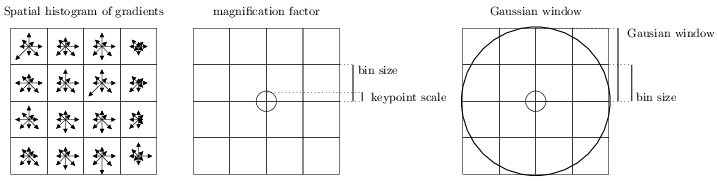
\includegraphics[width=0.6\textwidth]{image6.png}
%	\caption{Training error (left) and test error (right) on CIFAR-10 with 20-layer and 56-layer "plain" networks reproduced from XXXX }
%	\label{figre6}
%\end{figure}


The ResNet technique has shown deeper neural network models can train successfully. The model Microsoft used in ImageNet 2015 has 152 layers. That’s significantly deeper than previous competition winners. Deeper models tend to hit obstacles during the training process. The gradient signal vanishes with increasing network depth. But the identity connections in ResNets propagate the gradient throughout the model.

Researchers have hypothesized that deeper neural networks have more representational power. Deeper nets gain this power from hierarchically composing shallower feature representations into deeper representations. For instance, in face recognition, pixels make edges and edges make corners. Corners define facial features such as eyes, noses, mouths and chins. Facial features compose to define faces.

Which brings me to the first paper, Benefits of depth in neural networks by Matus Telgarsky. This paper shows mathematically that depth is necessary for representational power. It proves it for the class of activation functions common in deep learning research, such as rectified linear units (\textbf{ReLU}). Given a number k, there exist neural networks of depth $O(k^3)$, that are intractable. No depth k neural network can approximate them without exponentially many neurons $Ω(2^k)$. Thus, ResNets will be important to enable complex models of the world.

The second paper I’d like to highlight is Identity Mappings in Deep Residual Networks, by He et al. These are the original authors of the ResNet paper. The original technique only approximated identity connections between layers. Really, the layers still used nonlinear activations after the identity connections. These nonlinearities impede gradient propagation. The new paper runs with the identity connection concept. The signal propagates unchanged throughout the entire network. The activation functions between layers are absent. The new technique improves training and test performance.


%\begin{figure} \centering
%  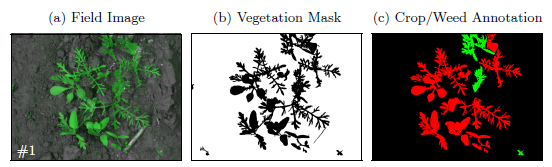
\includegraphics[width=0.9\textwidth]{image1.png}
%  \caption{Original versus proposed ResNet unit, and performance.}
%  \label{figsolplot}
%\end{figure}

The third paper is Resnet in Resnet: Generalizing Residual Architectures, by Targ et al. This paper experiments with additional complexity that runs parallel to the ResNet modules. Essentially, for every ResNet layer, they place a traditional convolutional layer next to it. They allow these parallel layers to exchange information. What results is a fractal ResNet structure. Groups of these modified ResNet modules can coordinate to learn longer-term ResNet structures.

%
%\begin{figure} \centering
%	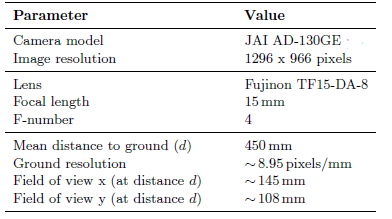
\includegraphics[width=0.9\textwidth]{image2.png}
%	\caption{ResNet in ResNet fractal structure.}
%	\label{figure2}
%\end{figure}


Next, is one of the most interesting papers I’ve seen: Deep Networks with Stochastic Depth, by Huang et al. This paper enables practical training of neural networks with thousands of layers. It modifies the technique dropout to remove layers from the network during training time. Entire layers get dropped at random. The remaining layers must compensate for their missing inputs by relying on lower inputs. Concretely, the technique sets the f(x) component to zero for several random layers, leaving the identity connections. Then the training procedure runs for a single step. Then those layers get reactivated while new ones get zeroed. During training, the depth of the network can be much smaller than normal. This results in fewer calculations and more efficient training throughput. The entire depth of the model is then used at inference time.

%
%\begin{figure} \centering
%	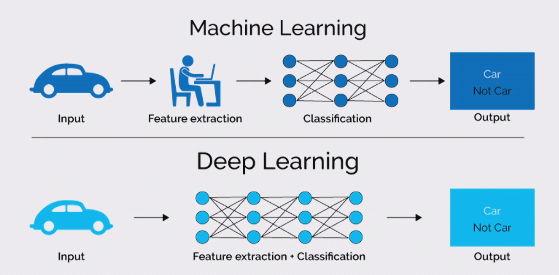
\includegraphics[width=0.9\textwidth]{image3.png}
%	\caption{Linear decay of layer dropout probabilities in stochastic depth.}
%	\label{figure3}
%\end{figure}


Another paper, Bridging the Gaps Between Residual Learning, Recurrent Neural Networks and Visual Cortex by Qianli Liao and Tomaso Poggio, explores the relationship between recurrent nets and residual nets. It augments recurrent nets with identity connections and shows such models have flexible topologies and improved performance. I find the techniques here to be very similar to two other papers: Neural GPUs Learn Algorithms by Łukasz Kaiser and Ilya Sutskever, and Adaptive Computation Time for Recurrent Neural Networks by Alex Graves.

Finally, the paper Deep Residual Networks with Exponential Linear Unit, by Shah et al., combines exponential linear units, an alternative to rectified linear units, with ResNets to show improved performance, even without batch normalization.

%\begin{figure} \centering
%	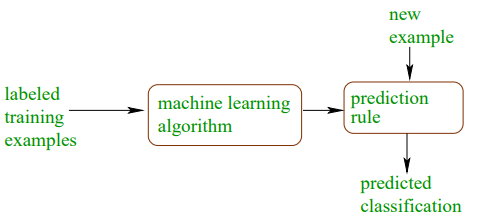
\includegraphics[width=0.9\textwidth]{image4.png}
%	\caption{Comparison of the learning behavior of (Auhor model) ant the original ResNet model on CIFAR-10 dataset}
%	\label{figure4}
%\end{figure}


%\subsection{Some Technicalities}
%Where to find this document? You may very well wonder about this point,
%if this document was given to you in paper form; if you downloaded it
%from my homepage, this will be obvious, of course. This document is
%available in the \LaTeX\ area of my homepage, which I will refer to
%as \cite{homepage} in the following.
%You will need to download several files, namely
%\verb+template.tex+, \verb+template.bib+, the three figures
%\verb+figconvrateloglog.jpg+, \verb+figconvrateplot.jpg+,
%and \verb+mesh_solution.jpg+, and the Matlab code \verb+plot_loglog.m+.
%
%How to read this document? Reading the resulting printout is useful,
%but you must also study carefully the \LaTeX-source code;
%I am trying to use all sorts of examples of sophisticated features.
%Notice how the result has a very simple appearance about it, but it takes
%some correct use of \LaTeX\ to achieve this goal at times.
%When reading the source code, pay particular attention, how all the
%referencing is done using the commands \verb+\label+ to set the label
%and \verb+\ref+ to refer to it. There are no separate labels or references
%for figures, tables, equations, sections, rather the meaning of the
%\verb+\label+ command is determined from the context, in which it appears.
%I have adopted the scheme to use the first three letters of the
%key for each label to indicate to myself, what kind of an object it
%refers to, so I use `fig' for figure labels, `tab' for table labels, etc.;
%see the source code.
% TMP
% How to create a printout of this document, though?
% See Section~\ref{secreferences} below.

%\subsection{Philosophy of this Document}

%This file is designed to show by
%example, how some relevant features of \LaTeX\ can be used to put
%together a technical report or a manuscript
%in such a form that it can be submitted to a journal.
%Any journal will have to work through your submission anyway, so
%it makes no sense to try to deal with some of the more technical
%requirements they have. Rather, your goal should be to provide clean
%\LaTeX, so that the copy editor only has to work on the formalities,
%but not the contents of the paper. In this spirit, it is very important
%that you provide information in expected places in some expected
%format; then the work of any editor is made easy. To this end, I
%am also trying to use clean but basic \LaTeX2$_\varepsilon$;
%this means that I am trying not
%to use any fancy features like redefining section headings,
%etc., but I allow myself the use of popular extensions that
%are available in packages that come with the standard distribution
%of \LaTeX\ under Linux.
%Again, if a journal wants the paper to look different,
%they will take care of that by using their macros.
%
%The additional purpose of this document is to demonstrate some of
%those more advanced of features of \LaTeX\ that are typically needed
%like importing figures or creating reference lists. For more basic
%commands, please see my basic sample document \emph{Some \LaTeX\ Introduction}
%\cite{homepage}; here and throughout, pay attention to my citations,
%as they are meant to show examples of how to cite certain types of
%publications. For more information about \LaTeX, you should consider
%\cite{Goossens94,Graetzer1996,Lamport94}.
%Leslie Lamport is the original creator of \LaTeX,
%and his book \cite{Lamport94}
%should be the starting point, in particular its Chapters~1 through~3
%\cite[Chapters~1--3]{Lamport94}.
%The other books \cite{Goossens94,Graetzer1996}
%are only needed for advanced uses of \LaTeX.
%Both books have similar content overall,
%but they have different approaches: \cite{Goossens94} is `horizontal'
%and discusses material organized by package; I suggest to use it,
%if you want to dig into the innards
%of \LaTeX\ like redefining section headers or advanced float placement.
%Compared to that, \cite{Graetzer1996} is organized `vertically,'
%because it discusses tools for one topic from all available sources together.
%If you need to typeset very complicted formulas or have other problems
%with the mathematics, I recommend \cite{Graetzer1996} because of its
%well-chosen examples and its organization.
%
%For an excellent discussion of writing mathematics in general, let me point
%to \cite{Higham98}. It contains more than the title lets on, namely
%also very relevant remarks on the politics of publishing in
%mathematics. If you are a Ph.D. student, you should definitely
%read this book.


\section{Deep Residual Networks} \label{secreferences}

For anyone serious about writing more than a single document, I urge
the use of the \textsc{Bib}\TeX\ bibliography system. Its complete
reference can be found in \cite[Appendix B]{Lamport94}.
In fact, even for a single document, it makes already sense to use it.
Let me explain both points presently.


\section{From 10 layers to 100 layers} \label{r1}

\section{From 100 layers to 1000 layers} \label{r2}

\textsc{Bib}\TeX\ is really a bibliography database system. Your whole
bibliography is contained in one or several files, in this case the file
\verb+template.bib+. In your text, you use then the \verb+\cite+ command
on the keys of those references. The point is that only those references
that you actually use get included in the references (note that for
instance the reference \verb+Gobbertiwce+ appears in the \verb+bib+-file
but not in the bibliography). To accomplish this,
you must run \LaTeX\ once to put all requested references in the
\verb+template.aux+, then run \textsc{Bib}\TeX\ once to pick up the
bibliographical information and create the file \verb+template.bbl+,
which contains the formated bibliography. Finally, you must run \LaTeX\
\emph{twice}: At first, it includes the bibliography in your document,
but during this first pass, it cannot have set the reference labels,
so in the second pass, the labels are correctly set. The upshot is,
always run \LaTeX\ twice to get all cross-referencing right. Remember
that this is needed whenever \emph{any} label or reference changes.
In summary, you should issue these commands:
\begin{verbatim}
  pdflatex template
  bibtex template
  pdflatex template
  pdflatex template
\end{verbatim}
Notice how \verb+plflatex+ is run \emph{twice} to get the cross-references
right. That is misleading, though, because you actually need to run
it \emph{three} times in total for this document
(which is done implicitly in the list above!),
if you want to get the formula reference right that appears in the caption
of Figure~\ref{figconvrateab}.

All this is started by the \verb+\bibliography{template}+ command
at the far end of this file; here, \verb+template+ refers to the file
\verb+template.bib+. Now, this is really a little unrealistic, because
the main advantage of \textsc{Bib}\TeX\ is that you can use one
\verb+bib+-file for all your research (or one per research project)
and maintain them at a central location. So, it is just done this way
here, so that you can download one simple file instead of my whole
bibliography database. Really, the following is my usual full command:
\begin{verbatim}
  \bibliography{/home/gobbert/soft/tex/biblio/curr/mgenmath,%
                /home/gobbert/soft/tex/biblio/curr/mreschem,%
                /home/gobbert/soft/tex/biblio/curr/mresmath,%
                /home/gobbert/soft/tex/biblio/curr/mresboltz}
\end{verbatim}
Actually, even this one is shortened to include only those \verb+bib+-files
related to that particular paper; I have more such files with bibliographical
information on other research projects.

What are the advantages of using \textsc{Bib}\TeX? I personally find
it actually easier to enter the information, hence I would even use it
for a single document. When entering it, I do not have to worry about the
referencing style required by the particular journal. Rather, \textsc{Bib}\TeX\
worries about that, when writing the \verb+bbl+-file. This appearance
is controlled by the \verb+\bibliographystyle{siam}+ command, where I
have chosen the referencing style for SIAM journals, which is one of
the standard ones supplied. So, here is the second advantage: You can
change the appearance of your bibliography merely by changing the
argument of the \verb+\bibliographystyle+ command. You may want to try
some other default ones like \verb+plain+ (which is pretty plain but elegant)
or \verb+ieeetr+ (which is quite nice).
Many journals supply their own bibliography style files,
such as \verb+nature+ or \verb+science+,
which you might need to download, since they are not part of the
standard distribution of \LaTeX.

Notice finally that the data in \verb+bib+-file(s) should be sensibly
arranged, for instance, alphabetically by the last name of the first
author; this order does not impact the order of appearance in your
document. A note on order might be in order: In engineering, you
often quote references by order of appearance, as you will see when
using \verb+ieeetr+. In mathematics, it is conventional to alphabetize
references by the last names of all authors, as is done by \verb+siam+.
Notice, how \cite{GoPr1} appears before \cite{Gobbert} independent of
chronology, but rather based on the last name of the second author.
(In fact, the order of the joint papers with Andreas Prohl is based on
alphabetizing the titles, which is quite non-sensical; if I did this
by hand, I would choose a chronological order.)

Other technical things include that several references together should
be referred to in one \verb+\cite+ command, namely as
\cite{Goossens94,Graetzer1996,Lamport94} and not as three citations
\cite{Goossens94}, \cite{Graetzer1996}, and \cite{Lamport94}.
Notice also that it does not matter if I say
\cite{Goossens94,Graetzer1996,Lamport94},
\cite{Graetzer1996,Goossens94,Lamport94}, or
\cite{Lamport94,Goossens94,Graetzer1996}, etc.;
see the source code to understand the difference between these
three citations!
That is accomplished by using the package \verb+cite+.
Notice that \verb+cite+ does some quite amazing things:
For instance, here are all publications cited in this template
that involve actual science (as opposed to \LaTeX\ and the like)
\cite{Gobbert,GoPr1,GoPr2,Gobbertima2000,Gobbertsiap2000,Ho95,Iserles96,RaimGobbert2010Poisson,Sharmathesis2010};
notice how \verb+cite+ groups the references without my doing
anything special; see the source code.

You might have noticed that the bibliography style \verb+siam+
uses all lowercase letters for the titles of articles.
That is not appropriate for proper names of software, places, or
natural persons that include Capital letters. In such cases,
you must inform \textsc{Bib}\TeX\ of these situations by putting
braces around either the letter or the word in question; see
\cite{Gobbertsiap2000} for an example.
It is also possible in the \verb+bib+-file to give \LaTeX\ commands like
\verb+\-+ to inform it of places for allowable hyphenation in a word that
it could not find by itself. That was done for the publisher of
\cite{Graetzer1996}.
% ; try processing this file without the \verb+\-+
% and you will get an \verb+Underfull \hbox+ warning.

I wanted to provide examples for the most common citations here.
So, for instance, \cite{Gobbertsiap2000} is the citation of a paper that
has been \emph{submitted} for publication. After acceptance, I would list
it as \emph{accepted} like \cite{Gobbertima2000}.
Finally, after I have received the page
proofs, I would list the paper as being \emph{in press} like \cite{GoPr2}.
(By the way, these papers are used as dummies here; they will remain
listed as submitted, accpeted, and in press in this template,
even once they appear.) On the other
hand, \cite{GoPr1} has appeared and shows all relevant information for
a journal article. For a book that appeared in a series,
\cite{Iserles96} would be an example (notice that this
one does not have a volume number in that series).
\cite{Sharmathesis2010} is the example of a M.S. thesis completed at UMBC,
and \cite{RaimGobbert2010Poisson} is a technical report.

Finally, let me discuss one kind of reference that causes regular
confusion on how to use correctly, namely the ``private'' or ``personal
communications.''
\cite{Ho95} is an example of how I have used this category in the past myself;
the point was that we used chemical formulas that were only
available to us as copy of transparencies. A more typical application
would be, if you have an e-mail exchange with a famous and distant researcher
as I am characterizing in \cite{BigShot}. I hope this helps to clear
up some confusion on the issue. If in doubt, ask your advisor for advice.

\section{Applications} \label{applications}
%http://kaiminghe.com/ilsvrc15/ilsvrc2015_deep_residual_learning_kaiminghe.pdf

%http://kaiminghe.com/icml16tutorial/index.html

%http://www.vision.ee.ethz.ch/ntire17/

%https://github.com/KaimingHe/deep-residual-networks#third-party-re-implementations

\section{Q \& A} \label{qa}

\section{Approach} \label{approach}


\section{Conclusions}

Deeper neural networks are more difficult to train \cite{Zagoruyko2016}






\section*{Acknowledgments}

To Maria Trujillo Ph.D., a teacher in the course fundamentals of multimedia machine learning for its valuable recommendations and its contributions along the semester fall 2017.
 
%\appendix


\bibliographystyle{siam}
\bibliography{template}

\end{document}

